% =====================================================================
%  Eigenes Foto der Stickmaschine im FabLab mit nummerierten Teilen.
%  Koordinaten relativ zum Foto: (0,0) unten links, (1,1) oben rechts.
%  Nummern wie in der Tabelle in Einweisung_Stickmaschine.tex
% =====================================================================
% \fotonr{Nummer}{Position der Nummer}{Bauteil}, nur innerhalb eines Foto-Scopes
\newcommand{\fotonr}[3]{%
  \draw[white, line width=2pt, line cap=round] (#2) -- (#3);
  \draw[black, line width=0.8pt] (#2) -- (#3);
  \fill[black] (#3) circle[radius=0.7mm];
  \node[marke, minimum size=5.5mm, font=\small\bfseries, line width=1pt] at (#2) {#1};}

\begin{tikzpicture}
  \node[anchor=south west, inner sep=0pt] (a) at (0,0)
    {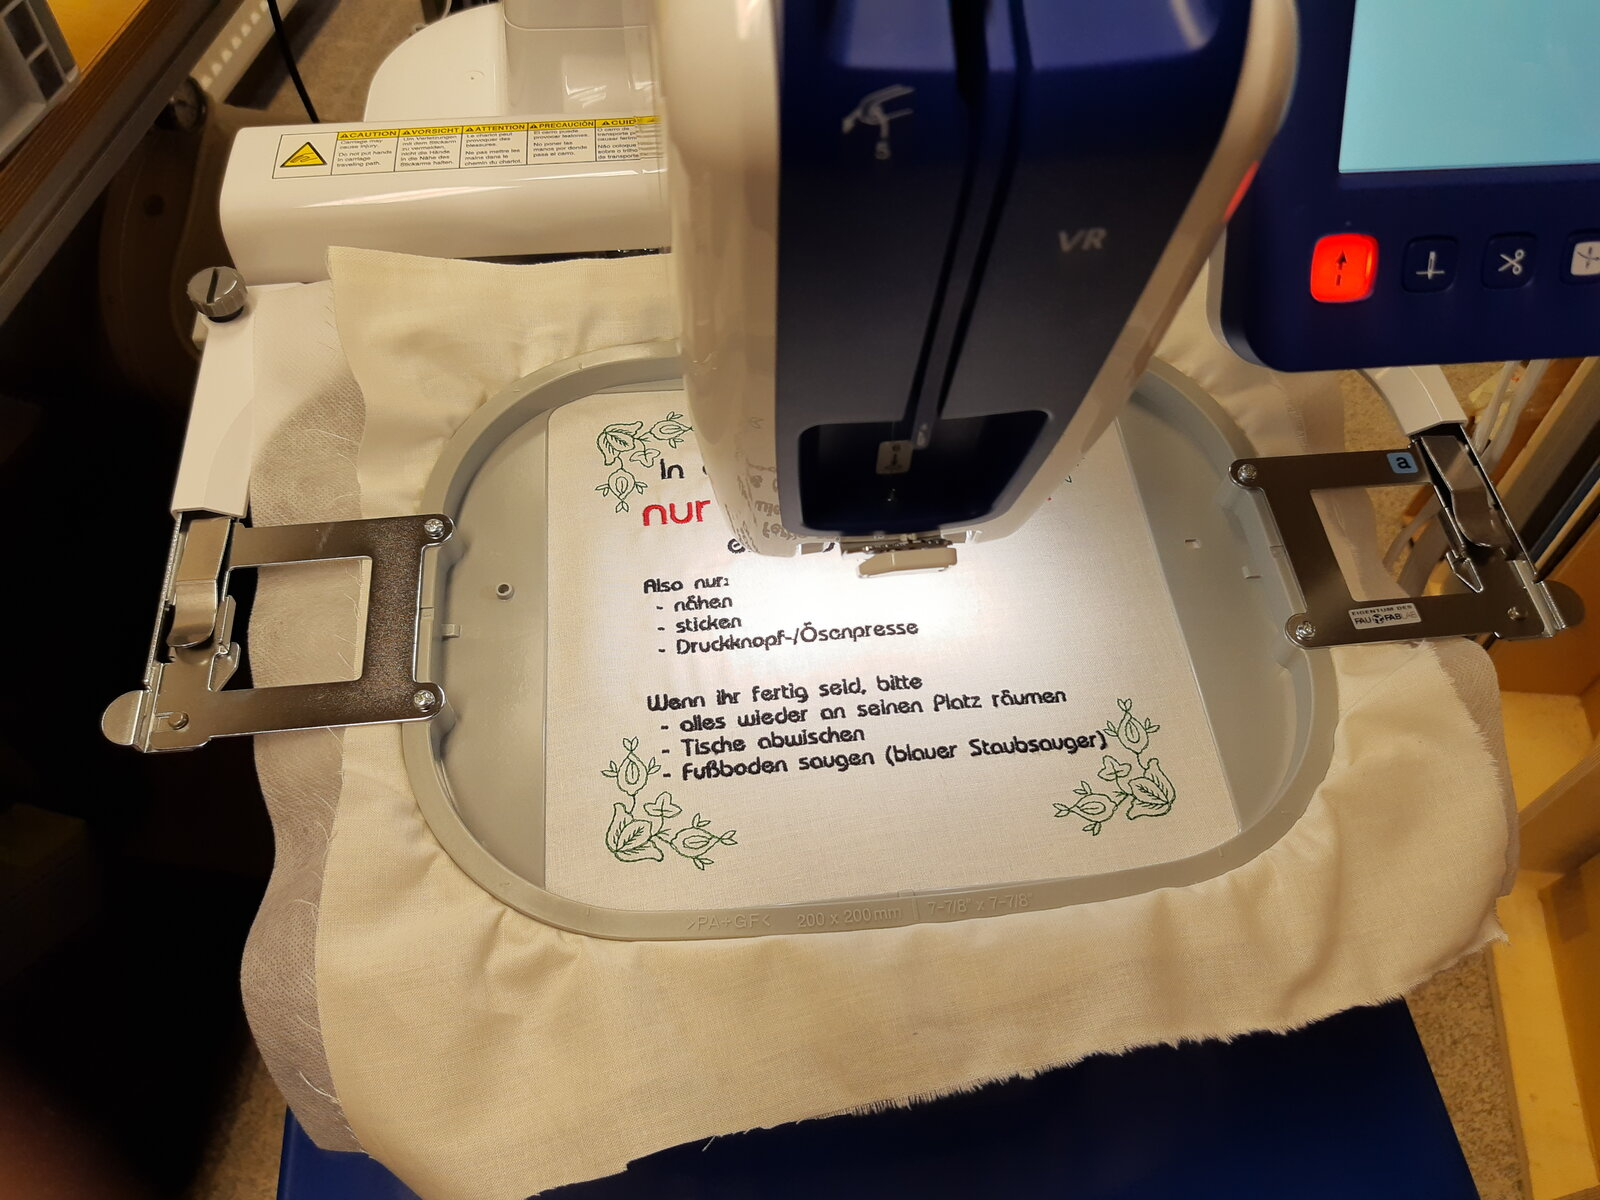
\includegraphics[width=0.92\textwidth]{bilder/stickmaschine-rahmen-gross.jpg}};
  \begin{scope}[x={(a.south east)}, y={(a.north west)}]
    \fotonr{1}{0.70,0.96}{0.90,0.93}   % Display
    \fotonr{2}{0.80,0.60}{0.839,0.779} % Start/Stopp
    \fotonr{3}{0.89,0.60}{0.894,0.779} % Nadelposition
    \fotonr{4}{0.97,0.92}{0.944,0.781} % Fadenabschneider
    \fotonr{5}{0.04,0.93}{0.286,0.857} % Stickarm
    \fotonr{6}{0.04,0.70}{0.136,0.762} % Rändelschraube Stickrahmenhalter
    \fotonr{7}{0.04,0.40}{0.150,0.467} % linker Arm des Stickrahmenhalters
    \fotonr{8}{0.96,0.40}{0.875,0.614} % Lasche am Rahmen
    \fotonr{9}{0.30,0.10}{0.40,0.243}  % Stickrahmen
    \fotonr{10}{0.36,0.70}{0.557,0.533}% Stickfuß und Nadel
  \end{scope}
\end{tikzpicture}
